\section{Presentation}
I'm an electronic engineer from School of Engineering and Technology ITBA,
recently graduate as Specialist in Embedded Systems and studying a
Master in Embedded Systems from University of Buenos Aires, UBA.\\
I developed my career working in product development area of several
national companies and in research in state institutions.\\
I was in charge of an electronic engineering studio offering electronic design
and production services and I am currently working as a freelance electronic
developer. \\ %with the possibility of issuing 'A' and 'B' invoices.\\ no da poner en ingles esto\ldots
I work daily designing embedded electronic equipment executing tasks such as: \\
\cvlistitem{Taking requirements and planning acceptance tests of hard and soft.}
\cvlistitem{Schematic design, PCB, simulations, assembly, 3D modeling and machining.}
\cvlistitem{Coding for real time in C / C ++ in bare metal or over RTOS.}
\cvlistitem{Bash and Python scripting over Linux and embedded Linux.}
\cvlistitem{Codification and execution of the unit tests and management of continuous integration tools.}
\cvlistitem{Assembly and start-up of prototypes and assembly line documentation.}
I am very pragmatic, committed and enjoy solving complex problems in a creative way by exchanging ideas
with my peers I prefer down-top developments using Agile concepts to keep the product functional from
the beginning.\\
I have an electronics workshop showed in figure \ref{fig:ofi_dci} and in the \href{\linkofidci}{video}, with tools as:\\
\cvlistitem{Assembly line of SMD/TH plates, pasta stencil, pick and place, reflow oven and wave soldering machine.}
\cvlistitem{Reworking and manual welding tools.}
\cvlistitem{Stock of SMD and TH materials of current and specific use.}
\cvlistitem{CNC machining center.}
\cvlistitem{Machine for cutting and laser engraving.}
\cvlistitem{Several machines for 3D printing.}
\cvlistitem{Generators, Oscilloscopes and Advanced Instrumentation for measurement and diagnosis.}
\cvlistitem{Electronic tools for firmware development.}
These tools, my experience, technical ability and frequent academic updating allow me to unwrap
in most instances of the development of a professional embedded electronic equipment.\\
Just follow the links in each section to see videos pdf's and detailed information.\\
You could check my up-to-date resume \href{\linkgithubcvpdf}{here}.\\

  \begin{figure}
      \begin{center}
         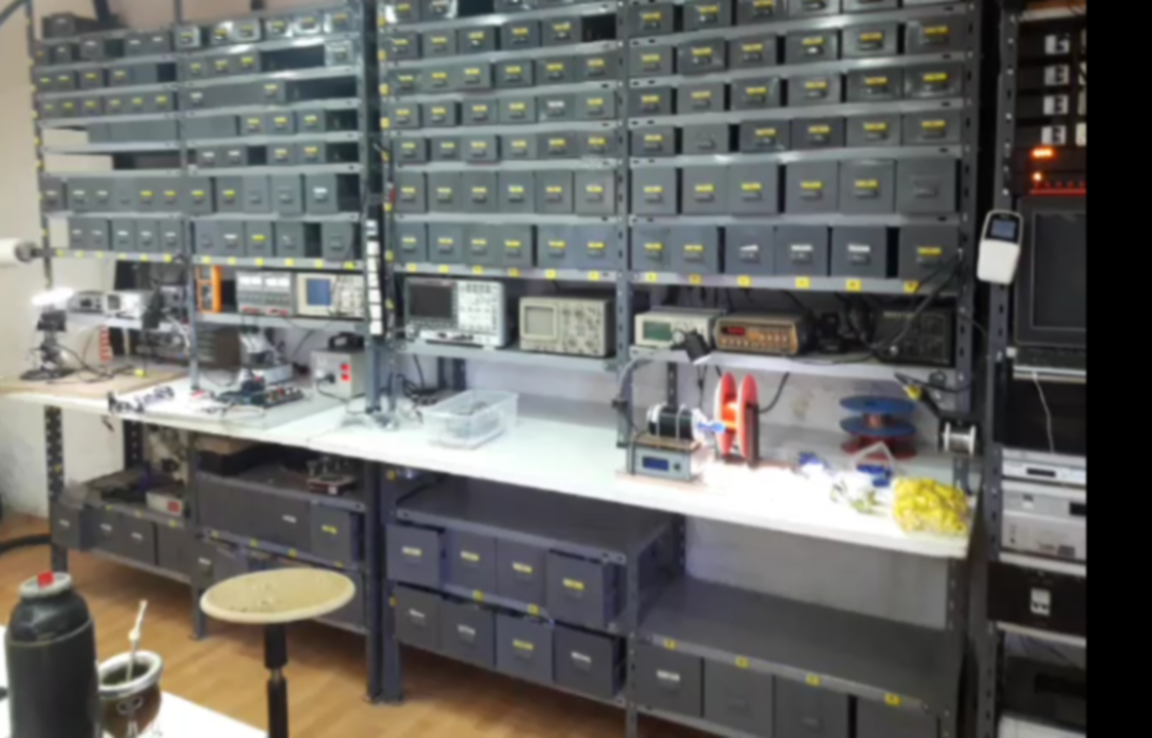
\includegraphics[width=0.3\textwidth]{ofi_dci1.png}
         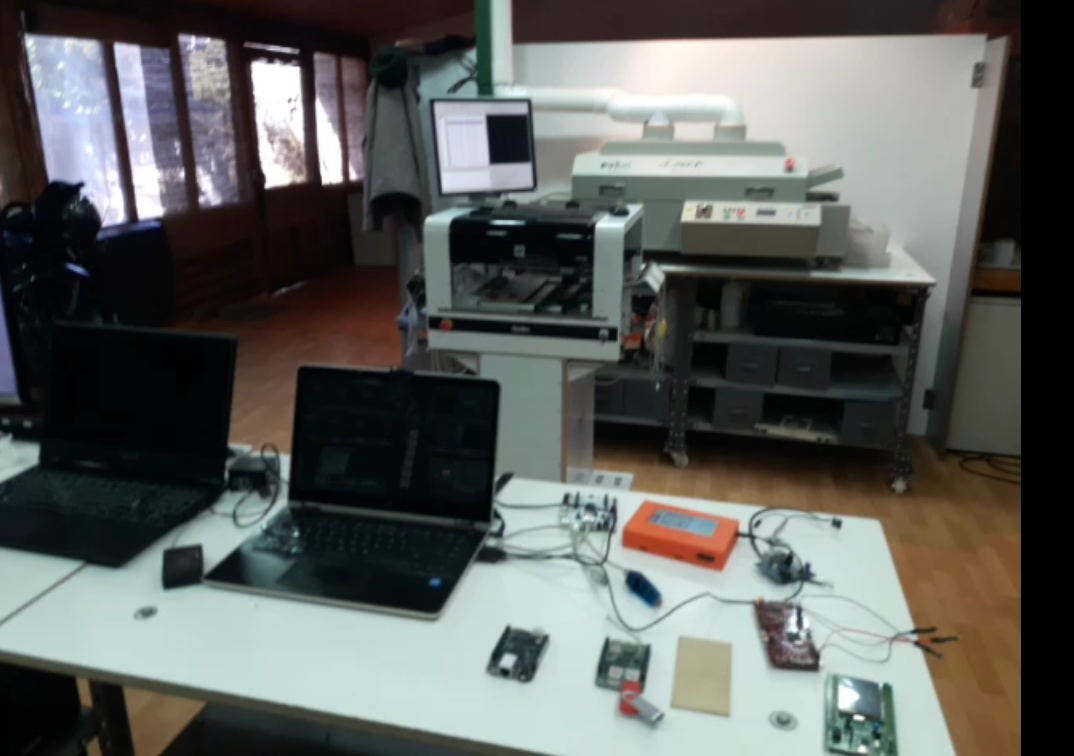
\includegraphics[width=0.3\textwidth]{ofi_dci2.png}
         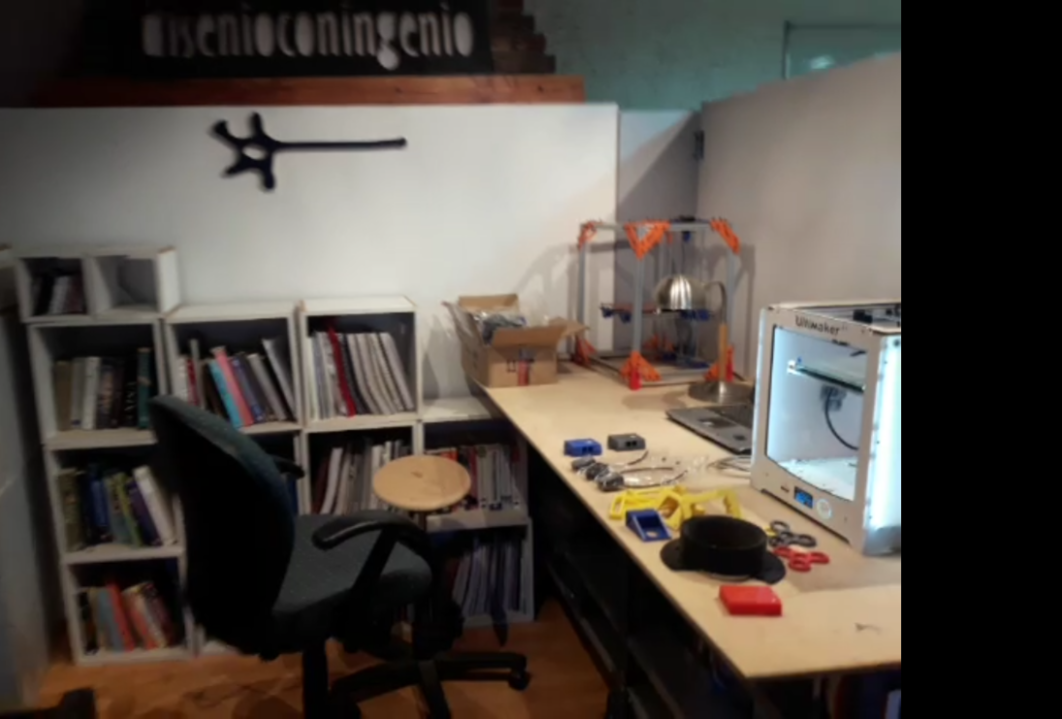
\includegraphics[width=0.3\textwidth]{ofi_dci5.png}
      \end{center}
      \caption{Development lab at Bariloche, 2019}
      \label{fig:ofi_dci}
   \end{figure}
